\section{Protocol}

Each command is termintad by a newline character, and each value in a command is separated by a whitespace.

Overview of packets:
\begin{table}[h!]
	\centering
	\label{Protocol:overview}
	\begin{tabular}{l|llll}
		\# & Description 		& Commando    		& Direction             & Example     		\\\hline
		0  & Handshake   		& RollingRoad 		& PC $\rightarrow$ PSoC & 0 RollingRoad 	\\
		1  & Unit description 	& <int> <str> <str> & PSoC $\rightarrow$ PC & 1 0 Time Seconds 	\\
		2  & Stop        		&            		& PC $\rightarrow$ PSoC	& 2        			\\
		3  & Information 		& <double> ... <double>	& PSoC $\rightarrow$ PC & 3 2 3 	    	\\
		4  & Torque control 	& <double>    			& PC $\rightarrow$ PSoC & 4 2.5  				\\
	\end{tabular}
	\caption{Overview for commands sent between PSoC og PC}
\end{table}

The table \ref{Protocol:overview} will give an on overview regardring the protocol that will be used between PC and PSoC. The chosen protocol will always start by sending an integer that corresponds with the given number from the above table.  The next thing that will be send is the column "Commando" that corresponds with the given number. The direction column shows the direction of the signals, where from and where to the signal will flow.      

In figure \ref{fig:TimingDiagram}, the flow of communication can be seen. Starting with the handshake initiated by the PC, followed by the PSoC repeating. After the handshake, the PSoC transmits all type and units this source can collect.

\fixme{Flip handshake direction}
\begin{figure}
\centering
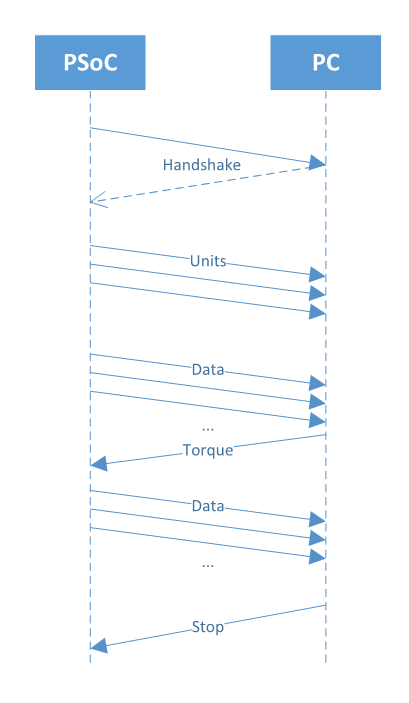
\includegraphics[width=0.5\linewidth]{Protocol/TimingDiagram}
\caption{}
\label{fig:TimingDiagram}
\end{figure}


\fixme{Create in-depth description of each}